\section{SimSite3D::geometry::vertex\_\-t Class Reference}
\label{classSimSite3D_1_1geometry_1_1vertex__t}\index{SimSite3D::geometry::vertex_t@{SimSite3D::geometry::vertex\_\-t}}
Might be better named \char`\"{}node\char`\"{}?  


{\tt \#include $<$Tri\-Mesh\-Sphere.H$>$}

Inheritance diagram for SimSite3D::geometry::vertex\_\-t::\begin{figure}[H]
\begin{center}
\leavevmode
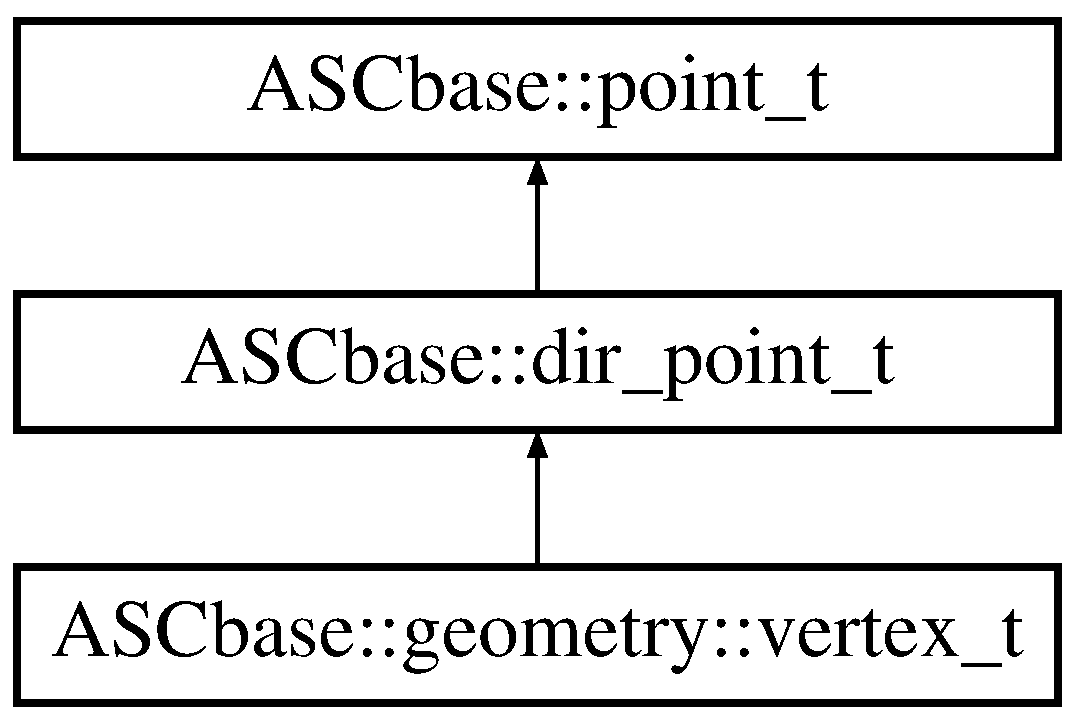
\includegraphics[height=3cm]{classSimSite3D_1_1geometry_1_1vertex__t}
\end{center}
\end{figure}
\subsection*{Public Member Functions}
\begin{CompactItemize}
\item 
\textbf{vertex\_\-t} (alloc\_\-t a=ALLOC\_\-POSITION)\label{classSimSite3D_1_1geometry_1_1vertex__t_b26d405918f18263845710e1cbdbd478}

\item 
\textbf{vertex\_\-t} (const \bf{vertex\_\-t} \&v)\label{classSimSite3D_1_1geometry_1_1vertex__t_369761b4291cb2a821f12dd56e409eb7}

\item 
const \bf{vertex\_\-t} \& \textbf{operator=} (const \bf{vertex\_\-t} \&v)\label{classSimSite3D_1_1geometry_1_1vertex__t_9073d65a8993b63729b0ddea759c7cd6}

\item 
void \textbf{setup\_\-one\_\-ring} (half\_\-edge\_\-vci beg\_\-in, half\_\-edge\_\-vci end\_\-in)\label{classSimSite3D_1_1geometry_1_1vertex__t_10f4bc8c2b1f885ebe29a995acdb3d31}

\item 
bool \textbf{inside\_\-one\_\-ring} (const my\_\-float\_\-t $\ast$pt)\label{classSimSite3D_1_1geometry_1_1vertex__t_107f530235423b366efbcd69c33d8f21}

\end{CompactItemize}
\subsection*{Private Attributes}
\begin{CompactItemize}
\item 
std::list$<$ half\_\-edge\_\-vci $>$ \textbf{A\_\-one\_\-ring\_\-edges}\label{classSimSite3D_1_1geometry_1_1vertex__t_9d8c7fb281ada6fd0369cda6007d3f55}

\end{CompactItemize}


\subsection{Detailed Description}
Might be better named \char`\"{}node\char`\"{}? 



The documentation for this class was generated from the following file:\begin{CompactItemize}
\item 
Tri\-Mesh\-Sphere.H\end{CompactItemize}
